 
   %judul bisa diketik ulang
  \setstretch{1}%\small
  \begin{center}
      \textbf{\large \Title}\\
      \bigskip 
  \end{center}
  
  
  
  %Nama authors
   \begin{center}
     \bf \Author$^1$, Didit Adytia$^2$
  \end{center}
  
  %Afiliasi dan email
   \begin{center}
     $^{1,2,3}$Fakultas Informatika, Universitas Telkom, Bandung\\
$^1$siswanto@students.telkomuniversity.ac.id, $^2$adytia@telkomuniversity.ac.id
  \end{center}
  
   
 %%% Abstrak Indonesia %%%%%%%%%%
   
{\bf \parindent0pt \noindent\rule{\textwidth}{1pt}
Abstrak

Prediksi \emph{runup} gelombang dapat dijadikan sebagai acuan bagi masyarakat yang berada di sekitar pesisiran pantai untuk melakukan mitigasi. Ketika gelombang mencapai ketinggian tertentu dapat membahayakan nyawa manusia dan menyebabkan kerusakan atau kerugian bagi manusia. Dengan adanya terumbu karang yang berada di pinggiran pantai energi dari gelombang teredam . Dalam jurnal ini akan dilakukan prediksi tinggi \emph{runup} gelombang di atas terumbu karang dengan menggunakan metode pembelajaran mesin \emph{Multi Layer Perceptron (MLP)} dengan 5 \emph{hidden layer}, 120 hidden layer jumlah neuron, dan 120 jumlah \emph{lookback}. Data yang digunakan adalah data dari hasil eksperimen yang dilakukan oleh Demirbilek pada tahun 2007 yang dilakukan pada laboratorium dinamika untuk meneliti redaman gelombang oleh terumbu karang. Berdasarkan hasil ujicoba dengan konfigrasi model terbaik berdasarkan optimasi \emph{hyperparameter}, pada data testing mendapatkan \emph{Mean Squared Error (MSE)} sebesar 0.113 sedangkan untuk data training dihasilkan MSE sebesar 0.024.\\

Kata kunci : Mitigasi, \emph{Runup}, \emph{Artificial Neural Network}, \emph{Multilayer perceptron}, Percobaan guam.

%%% Abstrak English %%%%%%%%%%  

\noindent\rule{\textwidth}{1pt}
Abstract

Runup prediction can be used by nearshore population to do disaster mitigation. When the nearshore waves reached certain height, it may endanger human lives, and causes severe damage to buildings. The existence of fringing reef can reduce the wave energy comming from the sea. This paper is using artificial neural network to predict runup height, with 5 hidden layer, 120 neurons each layer, and 120 lookback . The data used in this paper is the laboratorium data from University of Michigan. Based on the hyperparameter optimization, the optimal model configuration has $MSE=0.113$ on testing data, and $MSE=0.024$ on training data.

 \bigskip
Keywords: Mitigation, Runup, Artificial Neural Network, Multilayer perceptron, Guam experiment

\noindent\rule{\textwidth}{1pt} }

%%%%%% isi paper %%%%

\section{Pendahuluan}
\subsection{\textbf{Latar Belakang}}

Terumbu karang adalah ekosistem bawah laut yang terbentuk dari sekumpulan karang. Selain berfungsi sebagai ekosistem di bawah laut, terumbu karang juga berfungsi sebagai pemecah gelombang. Sebagian besar kepulauan di wilayah pasifik di kelilingi oleh terumbu karang yang tumbuh di laut dangkal yang dekat dengan pantai \cite{DemirbilekBoussinesq}.

Gelombang yang melewati terumbu karang akan teredam kecepatannya \cite{DemirbilekReport}. Hal ini akan mempengaruhi naiknya gelombang ke daratan di atas batas normal gelombang \emph{runup}\cite{nielsen1991wave}. Teredamnya kecepatan gelombang disebabkan oleh bertumbukannya dasar gelombang dengan karang. Dalam beberapa kasus, hal ini menyebabkan pecahnya gelombang \cite{DemirbilekReport}. Pada Gambar.\ref{fig:hawai_coral} dapat dilihat pecahnya gelombang yang terjadi di atas karang.

\begin{figure}[htp]
    \begin{center}
        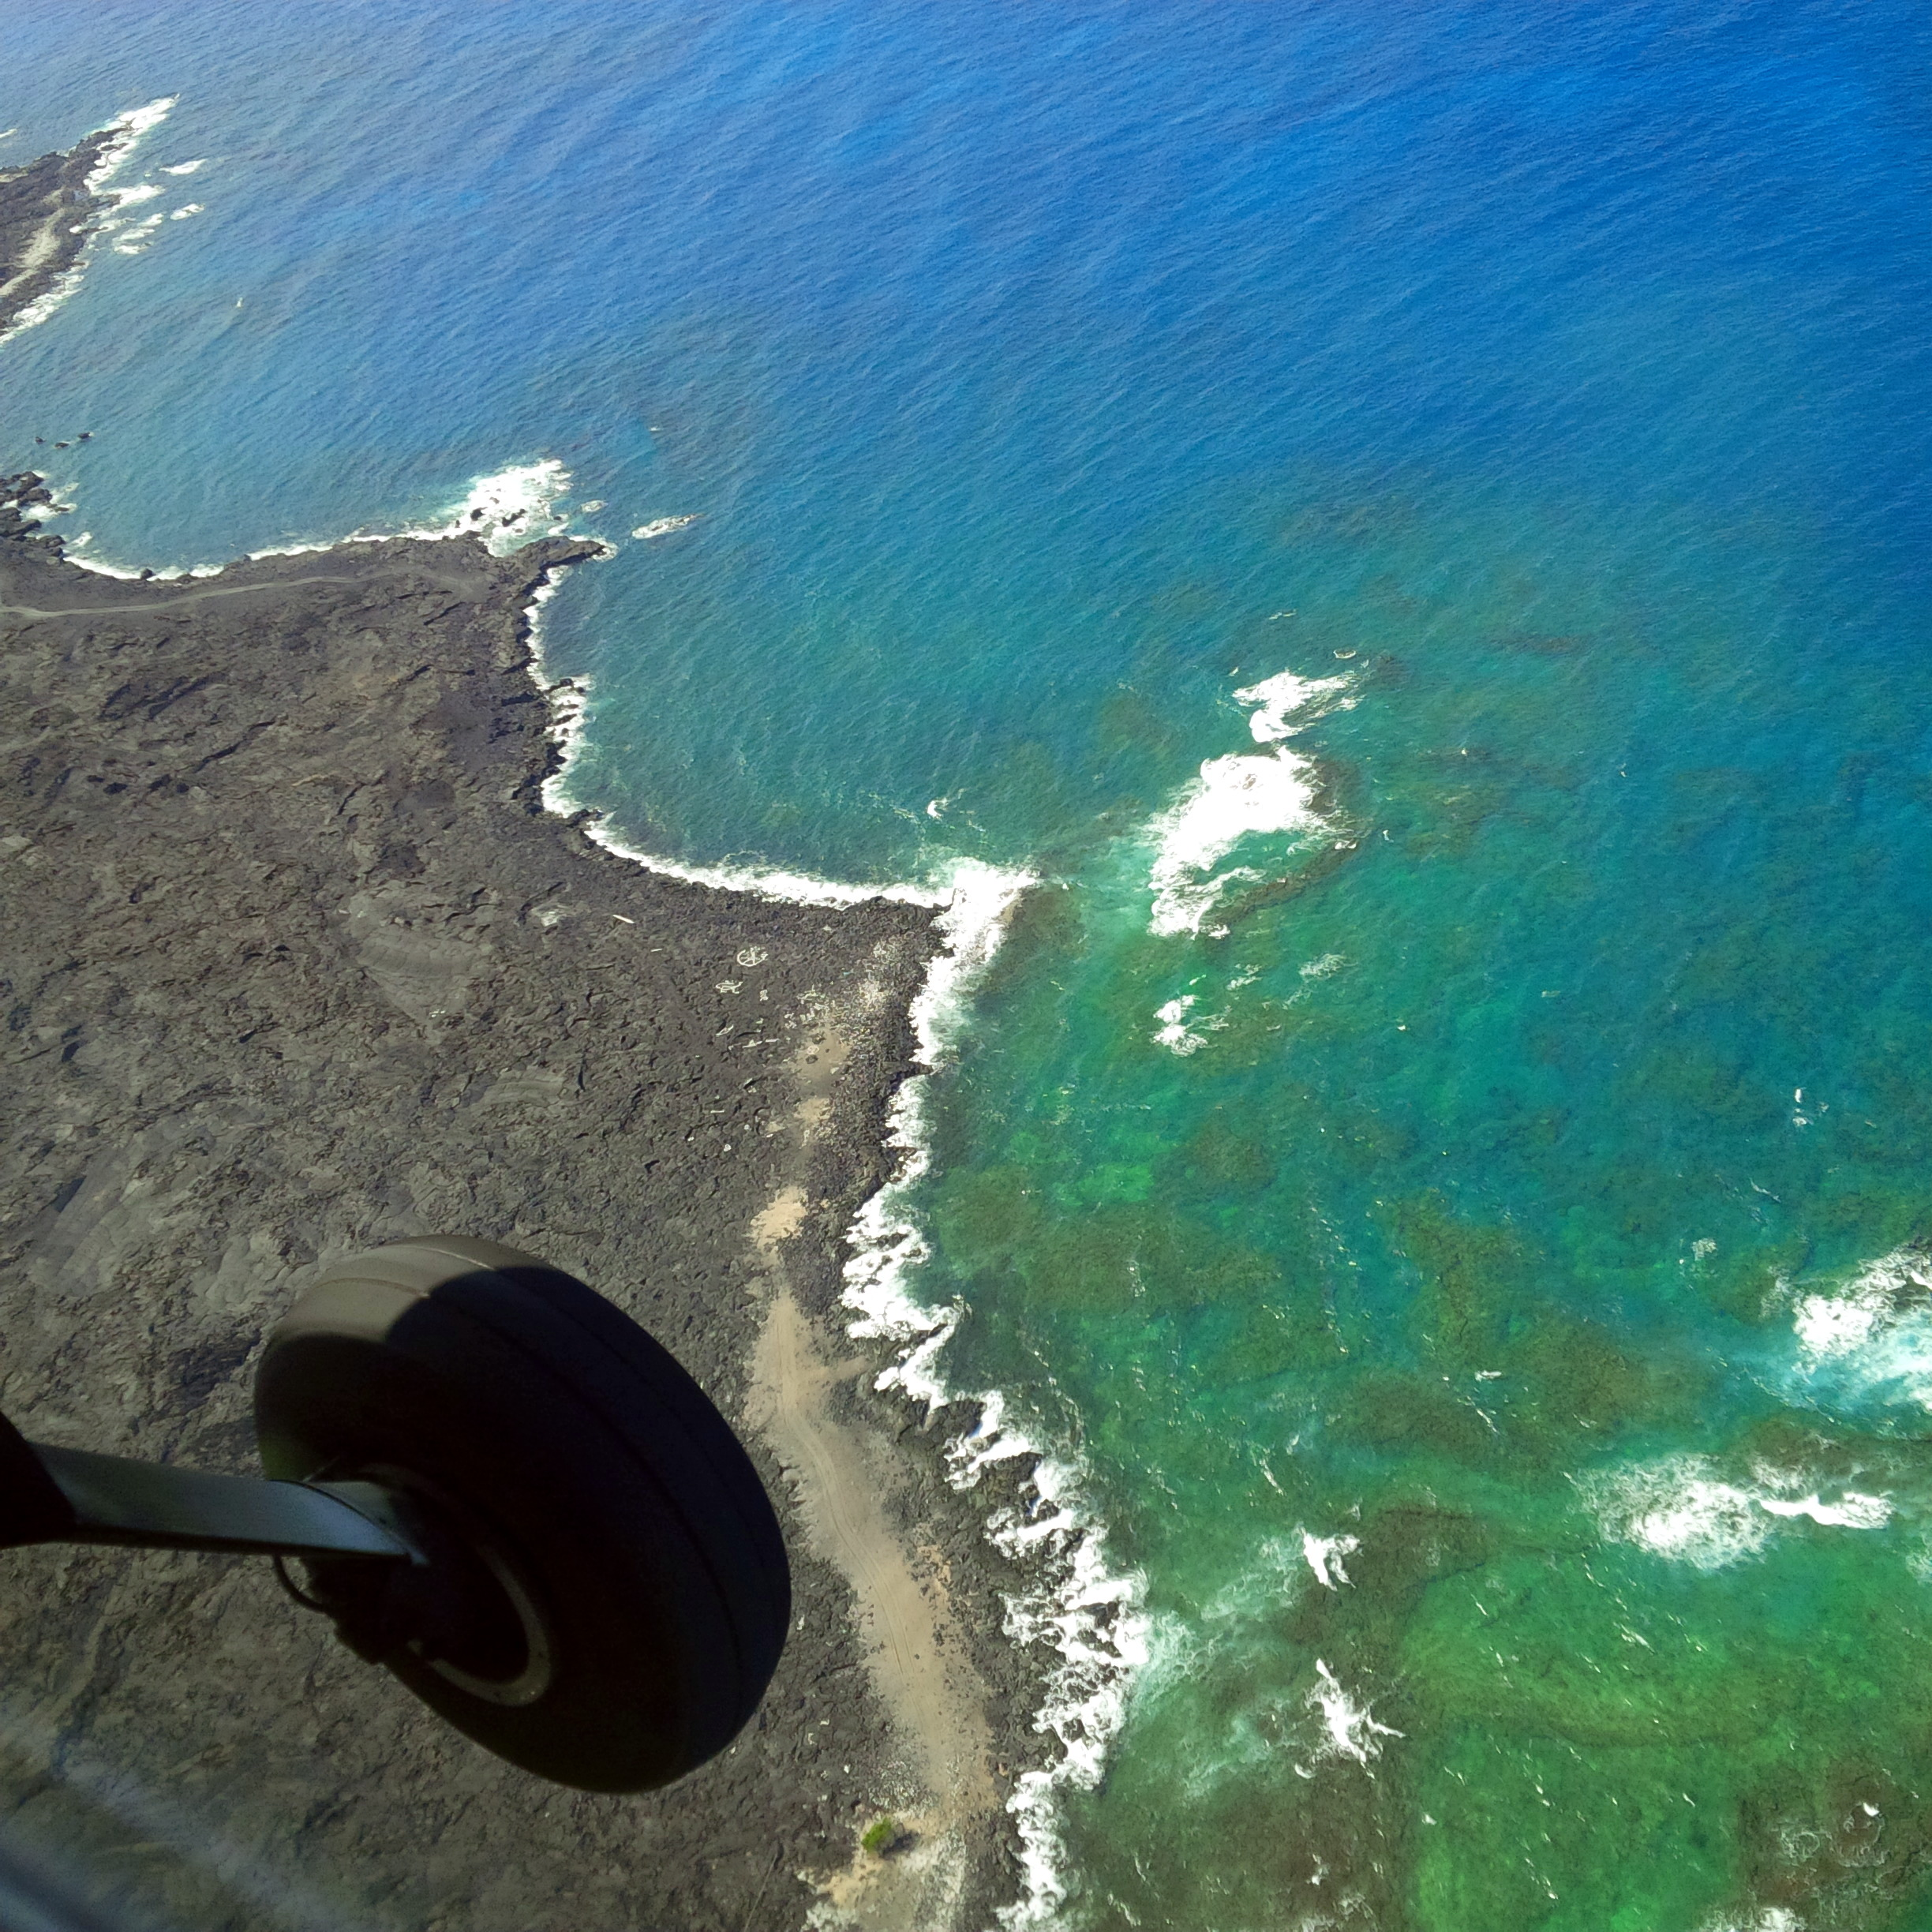
\includegraphics[scale=0.1]{./images/hawai_coral.jpg}
    \end{center}
    \caption{Terumbu Karang di tepi pantai di sekitar Hawai.}
    \label{fig:hawai_coral}
\end{figure}
\FloatBarrier
Efektifitas dari terumbu karang dalam meredam gelombang masih menjadi perdebatan para peneliti. penelitian ini sudah pernah dilakukan oleh Yau et al pada tahun 2012 dengan menggunakan model \emph{Boussinesq} 1 dimensi untuk memodelkan transformasi gelombang saat melewati terumbu karang. Namun cara mempelajari ini tergolong mahal dan membutuhkan pemodelan matematika yang kompleks untuk memodelkan pecahnya gelombang\cite{YAO201230}

Dalam memprediksi tinggi gelombang \emph{runup} pada terumbu karang digunakan dua metode yang masih tergolong baru yaitu metode pendekatan klasik yang dilakukan secara analitis yakni dengan melakukan eksperimen dan observasi kemudian, menentukan model matematika yang tepat. Model yang demikian sulit untuk dikembangkan karena beradaptasi dengan kondisi lingkungan yang berbeda. Prediksi yang didapat dari model yang demikian pun masih belum sempurna \cite{DemirbilekBoussinesq} Sedangkan metode yang kedua adalah dengan  pendekatan \emph{soft computing}.\\

{\textbf{Topik dan Batasan}}

Pada penelitian ini `menggunakan metode pembelajaran mesin yaitu dengan metode \emph{Feed forward neural network}(\emph{supervised learning}) untuk memprediksi tinggi \emph{runup} gelombang. data yang digunakan adalah data analisa observasi gelombang yang diambil dari laboratorium dinamika oleh Demirbilek pada tahun 2007\cite{DemirbilekReport}.\\

{\textbf{Tujuan}}

Tujuan dari tugas akhir ini adalah bagaimana membuat model \emph{Artificial Neural Network} (ANN) untuk memprediksi ketinggian \emph{runup} gelombang dengan menggunakan data hasil eksperimen pada laboratorium dinamika kemudian mengevaluasi hasil prediksi dengan mengevaluasi model dengan mencari nilai error dari model prediksi yang telah dibuat.



\section{Studi Terkait}
% Pembelajaran mesin sudah banyak dipakai di berbagai bidang keilmuan. seperti penelitian yang dilakukan oleh Lawrence  pada tahun 2007
% dengan judul 
% untuk mendeteksi wajah \cite{lawrence1997face}
% Mulai dari Pemrosesan citra seperti yang di lakukan oleh   . Dalam papernya dia menggunakan \emph{neural network} dengan tipe \emph{Convolutional Neural Network} untuk mendeteksi wajah. 

% Van Gent et al (2007) \cite{van2007neural}, 
% dia menggunakan \emph{Neural Network} untuk menganalisa \emph{overtopping} gelombang pada struktur di wilayah pantai. 

% Yau et al (2012)\cite{YAO201230}, dalam papernya dia menggunakan model \emph{Boussinesq} 1 dimensi untuk memodelkan transformasi gelombang ketika melewati terumbu karang. Pada bab ini dijelaskan model \emph{runup} gelombang pada terumbu karang menggunakan Pembelajaran Mesin.
\subsection{Runup Gelombang}
Runup gelombang adalah jarak vertikal maksimum dari kenaikan gelombang pada pantai atau struktur di atas \emph{SWL} \cite{sorensen2005basic}. Dalam penelitian ini, data ovservasi ketinggian \emph{runup} gelombang diukur mulai ketinggian \emph{swl}, hingga maksimum ketinggian air di daratan. Penjelasan lebih lanjut tentang pengambilan data dijelaskan pada bagian \nameref{kondisiEksperimen}. Runup gelombang dapat diilustrasikan pada gambar \ref{fig:runup}.
\begin{figure}[h]
    \begin{center}
        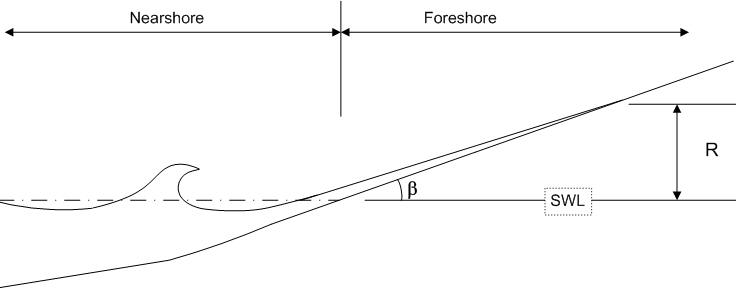
\includegraphics[scale=0.7]{./images/runup_gelombang.jpg}
    \end{center}
    \caption{Ilustrasi \emph{Runup} gelombang oleh Mike Swenson, Coastal Morphology, University of Wisconsin-Madison \cite{MikeSwenson:WaveRunup}.}
    \label{fig:runup}
\end{figure}
\FloatBarrier
Pada gambar.\ref{fig:runup} \emph{SWL (Sea Water Level)} adalah ketinggian air normal ketika tidak ada gelombang. Wilayah Pantai (\emph{Foreshore}) dimulai dari titik \emph{SWL} yang berpotongan dengan daratan. Wilayah lautan (\emph{Nearshore}) dimulai dari titik \emph{SWL} yang berpotongan dengan air. Ketika titik potong air dengan daratan berada di atas \emph{SWL}, maka kondisi tersebut dinamakan dengan \emph{runup}. Ketinggian \emph{runup} dinotasikan dengan $R$. Simbol $\upbeta$ melambangkan kemiringan bibir pantai.

\subsection{Pembelajaran Mesin}

Pembelajaran mesin adalah bidang studi yang memberikan kemampuan komputer untuk belajar, tanpa harus di program secara khusus \cite{arthur_l_samuel_1959}. Mesin dikatakan belajar dari pengalaman ($E$) terhadap tugas ($T$) dan ukuran kinerja ($P$), jika kinerja pada tugas ($T$), yang di ukur berdasarkan ($P$), berkembang berdasarkan pengalaman ($E$). Dalam TA ini, akan dibuat suatu program yang dapat belajar dari data gelombang hasil observasi ($T$). Lalu dievaluasi hasilnya dengan menggunakan $MSE$ ($P$), sehingga dapat di lihat seberapa besar galatnya. Lalu diperkecil galatnya dengan metode optimasi.

% \subsubsection{Supervised Learning}

% Sebelum data dimasukan ke dalam program, data tersebut diberikan label. Label tersebut bisa berupa \emph{input}, yakni $H$ (\emph{Significant Height} Gelombang), $T$ (\emph{Spectral Peak Periods}), dan $WL$ (\emph{Wave Length}). Dan label untuk \emph{output}. Karna pada TA kali ini, akan digunakan regresi linear. Maka tidak ada label untuk \emph{output}. Parameter \emph{input} yang berpasangan dengan \emph{output} tertentu, selanjutnya dinamakan contoh. Pembelajaran Mesin yang demikian dinamakan \emph{Supervised Learning}. \emph{Supervised Learning} Merupakan bagian dari pembelajaran mesin yang memetaan \emph{input} ke \emph{output} yang berdasar pada contoh pasangan \emph{input} dan \emph{output}\cite{AIPeterNorvig}. 

\subsubsection{Neural Network}

\emph{Neural network} pertama kali didefenisikan oleh McCulloch-Pitts pada tahun 1943 \cite{McCulloch1943}. \emph{Neural network} adalah model matematika atau model komputasi untuk memproses informasi berdasarkan pendekatan koneksionis ke komputasi, perilaku globalnya ditentukan oleh koneksi antara elemen pemrosesan dan parameter elemen\cite{gurney2014introduction}.
Arsitektur \emph{Neural network} terdiri dari \emph{Input neuron}, \emph{hidden layer} dan \emph{Output neuron}. Arsitektur \emph{Neural network} dapat dilihat pada gambar 
\ref{fig:neural_network_sederhana}

\begin{figure}[H]
    \centering
    \def\layersep{4cm}
    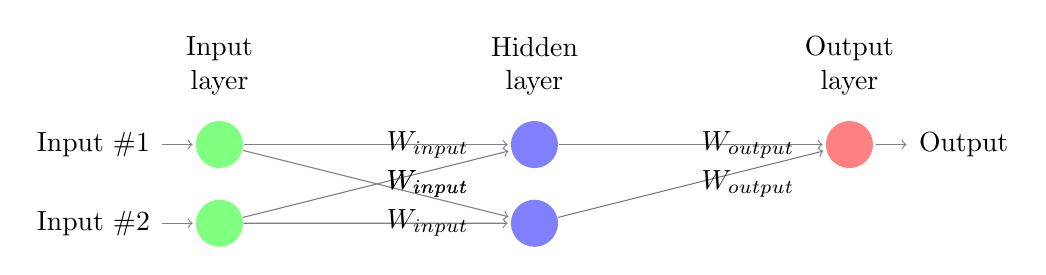
\begin{tikzpicture}[shorten >=1pt,->,draw=black!50, node distance=\layersep]
        \tikzstyle{every pin edge}=[<-,shorten <=1pt]
        \tikzstyle{neuron}=[circle,fill=black!25,minimum size=17pt,inner sep=0pt]
        \tikzstyle{input neuron}=[neuron, fill=green!50];
        \tikzstyle{output neuron}=[neuron, fill=red!50];
        \tikzstyle{hidden neuron}=[neuron, fill=blue!50];
        \tikzstyle{annot} = [text width=4em, text centered]

        % Draw the input layer nodes
        \foreach \name / \y in {1,...,2}
        % This is the same as writing \foreach \name / \y in {1/1,2/2,3/3,4/4}
            \node[input neuron, pin=left:Input \#\y] (I-\name) at (0,-\y) {};

        % Draw the hidden layer nodes
        \foreach \name / \y in {1,...,2}
            \path[yshift=0.0cm]{}
                node[hidden neuron] (H-\name) at (\layersep,-\y cm) {};

        % Draw the output layer node
        \node[output neuron,pin={[pin edge={->}]right:Output}, right of=H-1] (O) {};

        % Connect every node in the input layer with every node in the
        % hidden layer.
        \foreach \source in {1,...,2}
            \foreach \dest in {1,...,2}
                \path (I-\source) edge node[midway, right] {$W_{input}$} (H-\dest);

        % Connect every node in the hidden layer with the output layer
        \path (H-1) edge node[midway, right] {$W_{output}$} (O);
        \path (H-2) edge node[midway, right] {$W_{output}$} (O);

        % Annotate the layers
        \node[annot,above of=H-1, node distance=1cm] (hl) {Hidden layer};
        \node[annot,left of=hl] {Input layer};
        \node[annot,right of=hl] {Output layer};
        \label{neuralNetworkRepresentation}
    \end{tikzpicture}
    \caption{Model \emph{Neural Network} dengan 1 \emph{Hidden Layer}.}
    \label{fig:neural_network_sederhana}
\end{figure}

Pada umumnya persamaan \emph{Neural network} dapat dilihat pada pers.\ref{eq:regresi} dimana nilai z dapat dilihat pada pers.\ref{eq:mcullochNeuralNetwork}
\begin{equation}
    \label{eq:regresi}
    y = f(z)
\end{equation}

\begin{equation}
\label{eq:mcullochNeuralNetwork}
    z = \sum_{i=1}^N I_iW_i
\end{equation}

Dimana y adalah output, $I$ merupakan output dari neuron sebelumnya, $W_{i}$ adalah bobot atau \emph{Weight}, f(z) adalah nilai aktivasi dari hasil penjumlahan dari perkalian input dengan bobot. Fungsi aktivasi yang digunakan adalah fungsi aktivasi linear dan ReLU. 

\subsubsection{Fungsi Aktivasi}

Fungsi aktivasi digunakan untuk mengubah level aktivasi pada suatu neuron menjadi sebuah sinyal output \cite{KarlicOlgacPerformanceAnalysis}. Dalam penelitian ini fungsi aktivasi yang digunakan pada hidden layer adalah  fungsi aktivasi \emph{Rectified Linear Unit (RELU)}\cite{glorot2011deep}. Fungsi aktivasi \emph{RELU} didefinisikan dengan persamaan \ref{eq:aktivasi_relu}  dan fungsi aktivasi linear \cite{MLBishop}. pada pers.\ref{eq:aktivasi_linear}

\begin{equation} 
    \label{eq:aktivasi_relu}
ReLU (x)=\begin{cases} 0, & \mbox{if} x\le 0 \\ x, & \mbox{if} x > 0 \end{cases}
\end{equation}

\begin{equation}
    \label{eq:aktivasi_linear}
    y=x
\end{equation}

% RELU menjadi pilihan karna memiliki performa konvergensi yang lebih baik dibanding sigmoid \cite{Krizhevsky:2012:ICD:2999134.2999257}. 

\subsubsection{Estimasi Galat / \emph{Cost / Lost Function}}

Kalkulasi galat sangat penting untuk menentukan seberapa besar akurasi yang dimiliki model prediksi pada TA ini. Fungsi estimasi galat yang digunakan adalah \emph{Mean Square Error (MSE)}. Persamaan MSE didefinisikan dengan

\begin{equation}
    \operatorname{MSE}=\frac{1}{n}\sum_{i=1}^n(Y_i-\hat{Y_i})^2,
\end{equation}

dimana $Y$ adalah ketinggian gelombang hasil observasi, $\hat{Y}$ adalah ketinggian gelombang hasil prediksi, dan $n$ adalah jumlah data training.

% TODO:fix gambar instrumen eksperimen

\section{Sistem yang Dibangun}

Metode yang akan digunakan dalam penelitian ini adalah \emph{Artificial Neural Network} dengan menggunakan data hasil analisa yang dilakukan oleh Demirbilek pada tahun 2017\cite{DemirbilekReport}. Data tersebut dibagi menjadi 3 bagian, 70 persen data untuk testing, 15 persen data untuk validasi, 15 persen data untuk testing.

Sistem dimulai membaca data langsung dari file dan melakukan pre-processing, data lalu dimasukannya sebagai input ke dalam algoritma ANN untuk melakukan proses training. Konfigurasi model ANN untuk training dibentuk berdasarkan dari hasil optimasi hyperparameter. Setelah training, sistem akan menghasilkan suatu model yang berisi matriks $W$ dan $b (bias)$ di dalamnya.

\subsection{Data Set}
Data yang digunakan dalam penelitian ini adalah data dari eksperimen yang di lakukan oleh US Army Corps of Engineer pada Agustus - September 2006. Analisa dilakukan oleh Demirbilek et al dan di tulis dalam laporan yang berjudul \emph{"Laboratory Study of Wind Effect on Runup over Fringing Reefs"}. Data berasal dari hasil percobaan yang dilakukan di Ann Arbor oleh University of Michigan \cite{TechnicalReports}. Data memiliki format \emph{tab separated value (tsv)}, header sensor berlokasi di 
index ke 8 dari baris. Header 1 hingga 7 berisi meta informasi seputar data. Hanya meta informasi frequensi, channels, dan samples yang digunakan untuk jurnal ini. \emph{Channels} adalah jumlah row yang berisi data, \emph{Samples} adalah jumlah data, dan frequensi adalah jumlah \emph{sample} dari sensor yang diambil dalam waktu 1 detik. Masing-masing berfungsi untuk menentukan proses yang tepat dalam membaca data.
\FloatBarrier
\begin{figure}[h]
  \begin{center}
    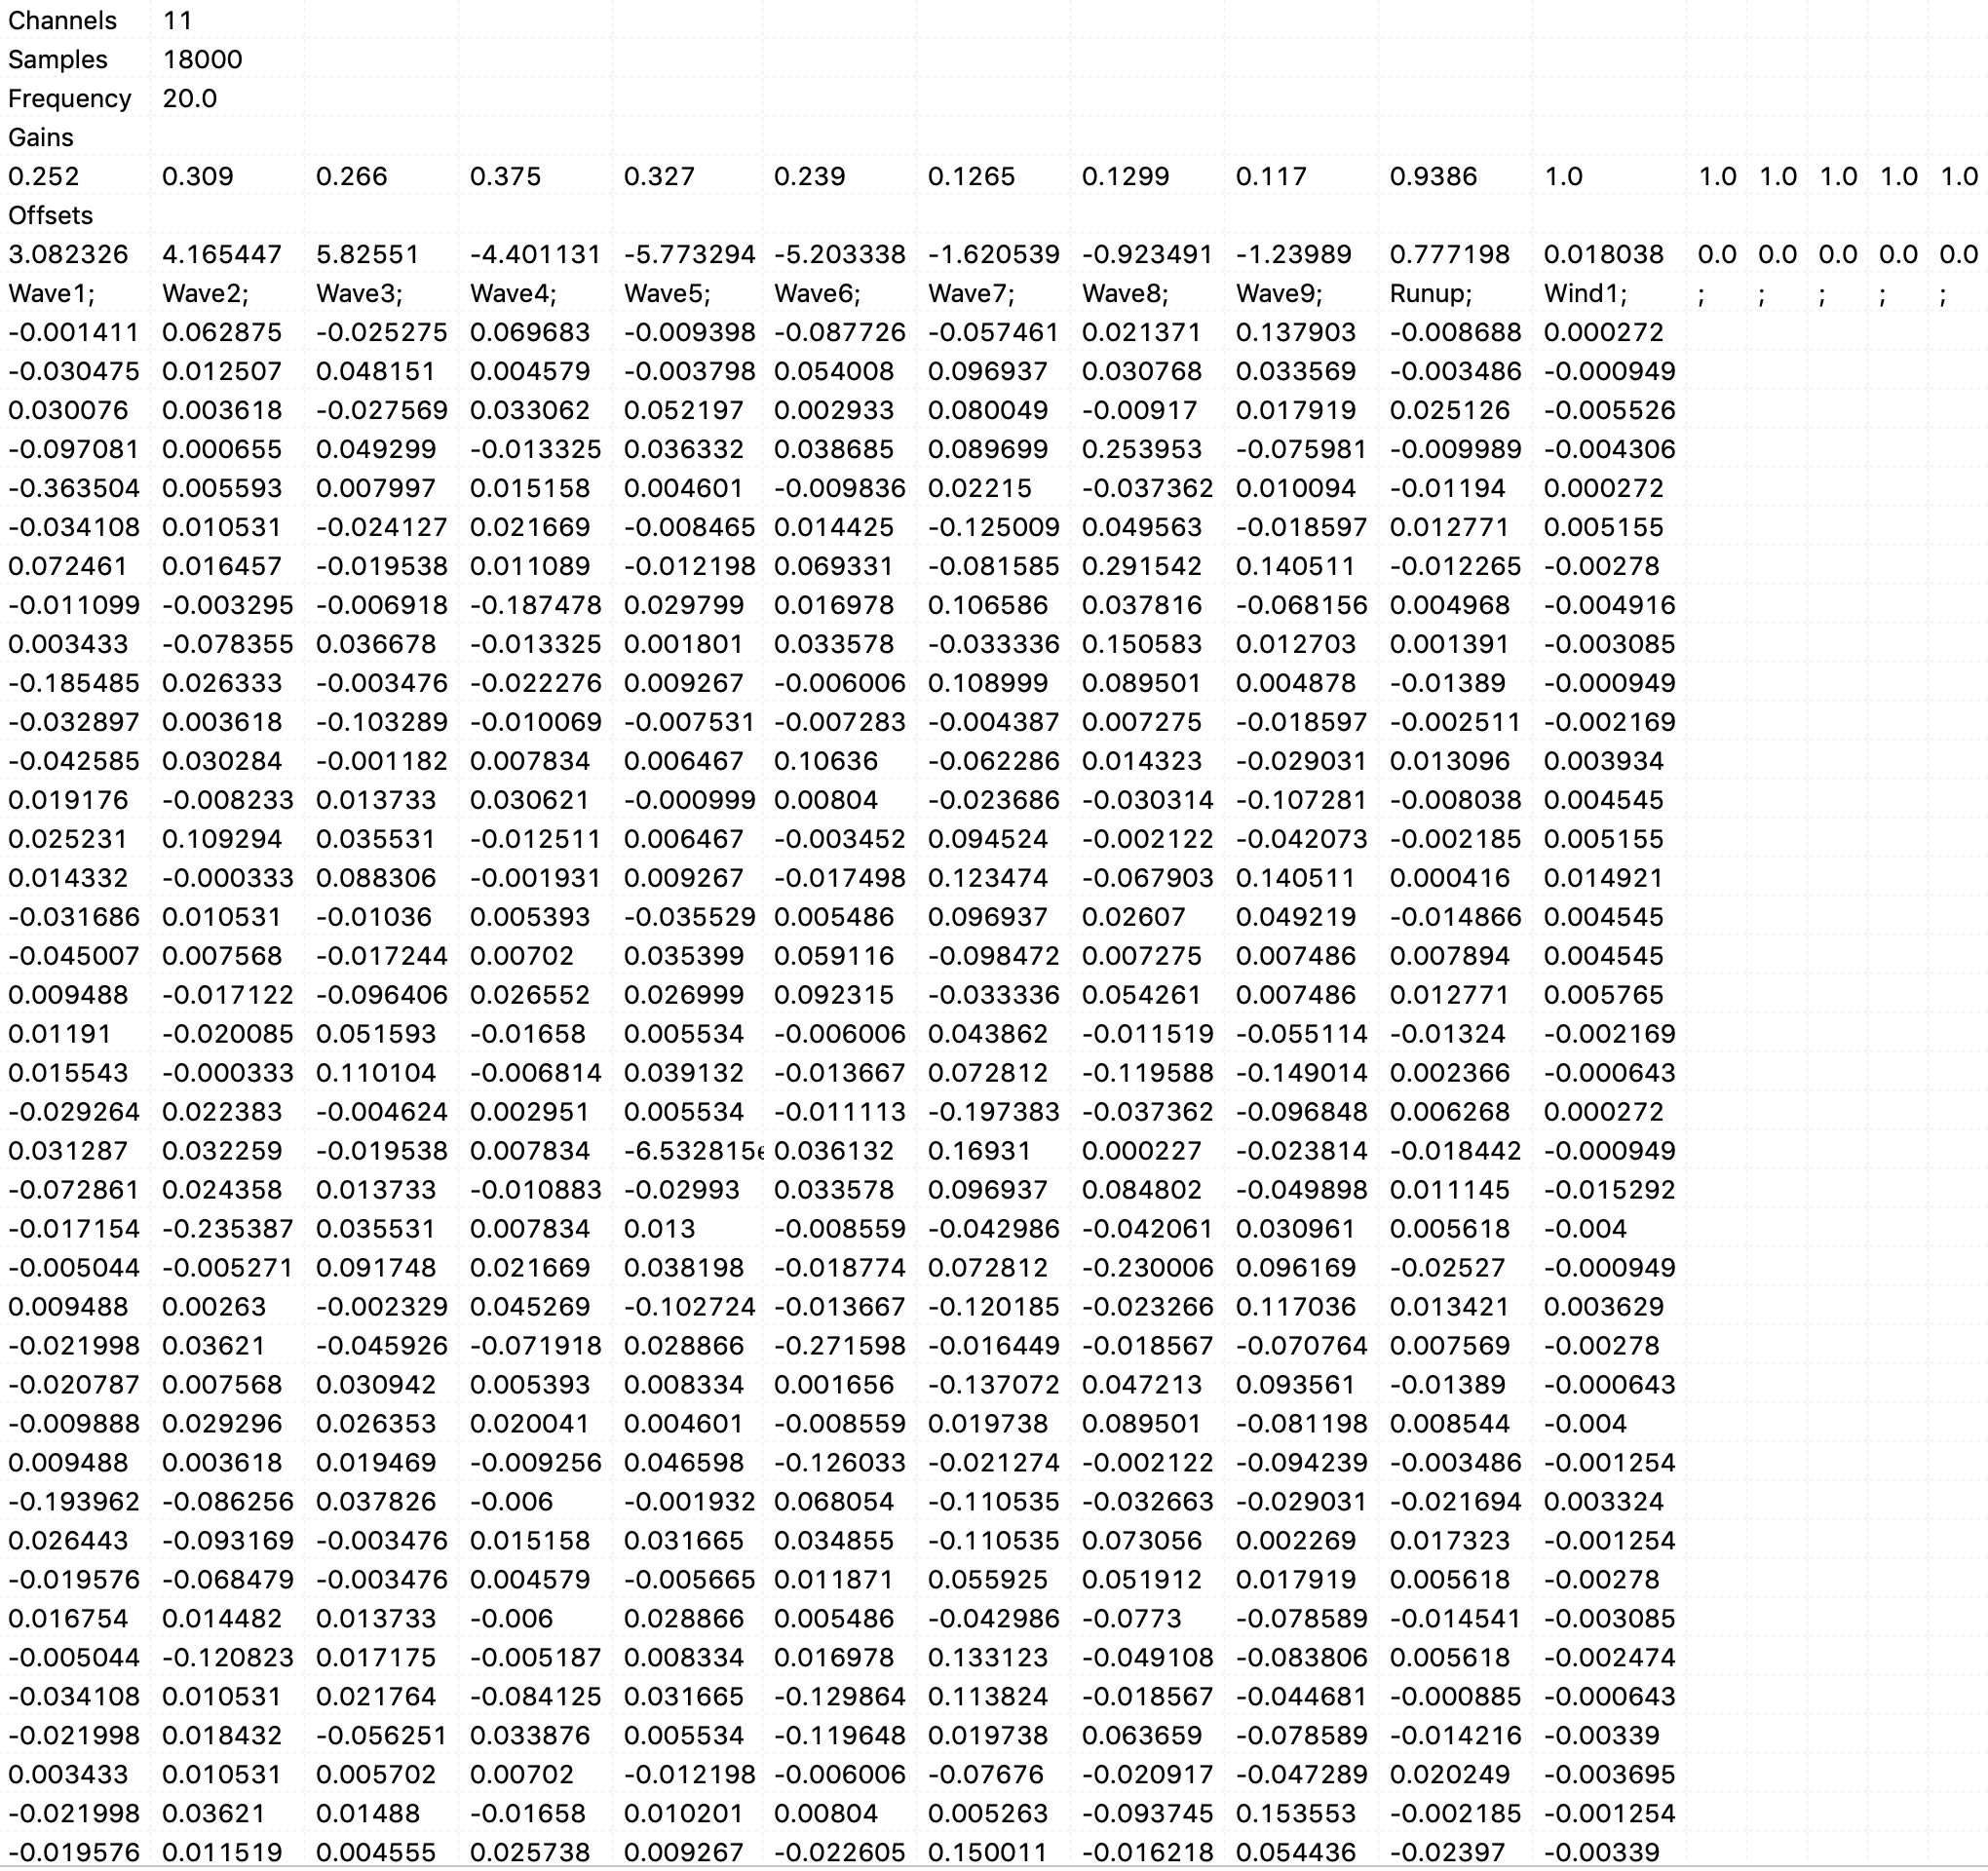
\includegraphics[scale=0.3]{./images/raw_data_test-18.png}
  \end{center}
  \caption{Raw data dengan nama file test-18.dat yang dihasilkan oleh percobaan di laboratorium.}
  \label{fig:raw_data_18}
\end{figure}
\FloatBarrier

\subsection{Kondisi Eksperimen}
\label{kondisiEksperimen}

Eksperimen dibagi menjadi 3 bagian. Eksperimen pertama dilakukan hanya menggunakan variabel gelombang dengan kecepatan angin 0. Eksperimen kedua dilakukan hanya menggunakan variabel angin. Selanjutnya eksperimen ketiga adalah gabungan dari perubahan variable gelombang dan variabel angin.

\begin{figure}[htbp!]
  \begin{center}
    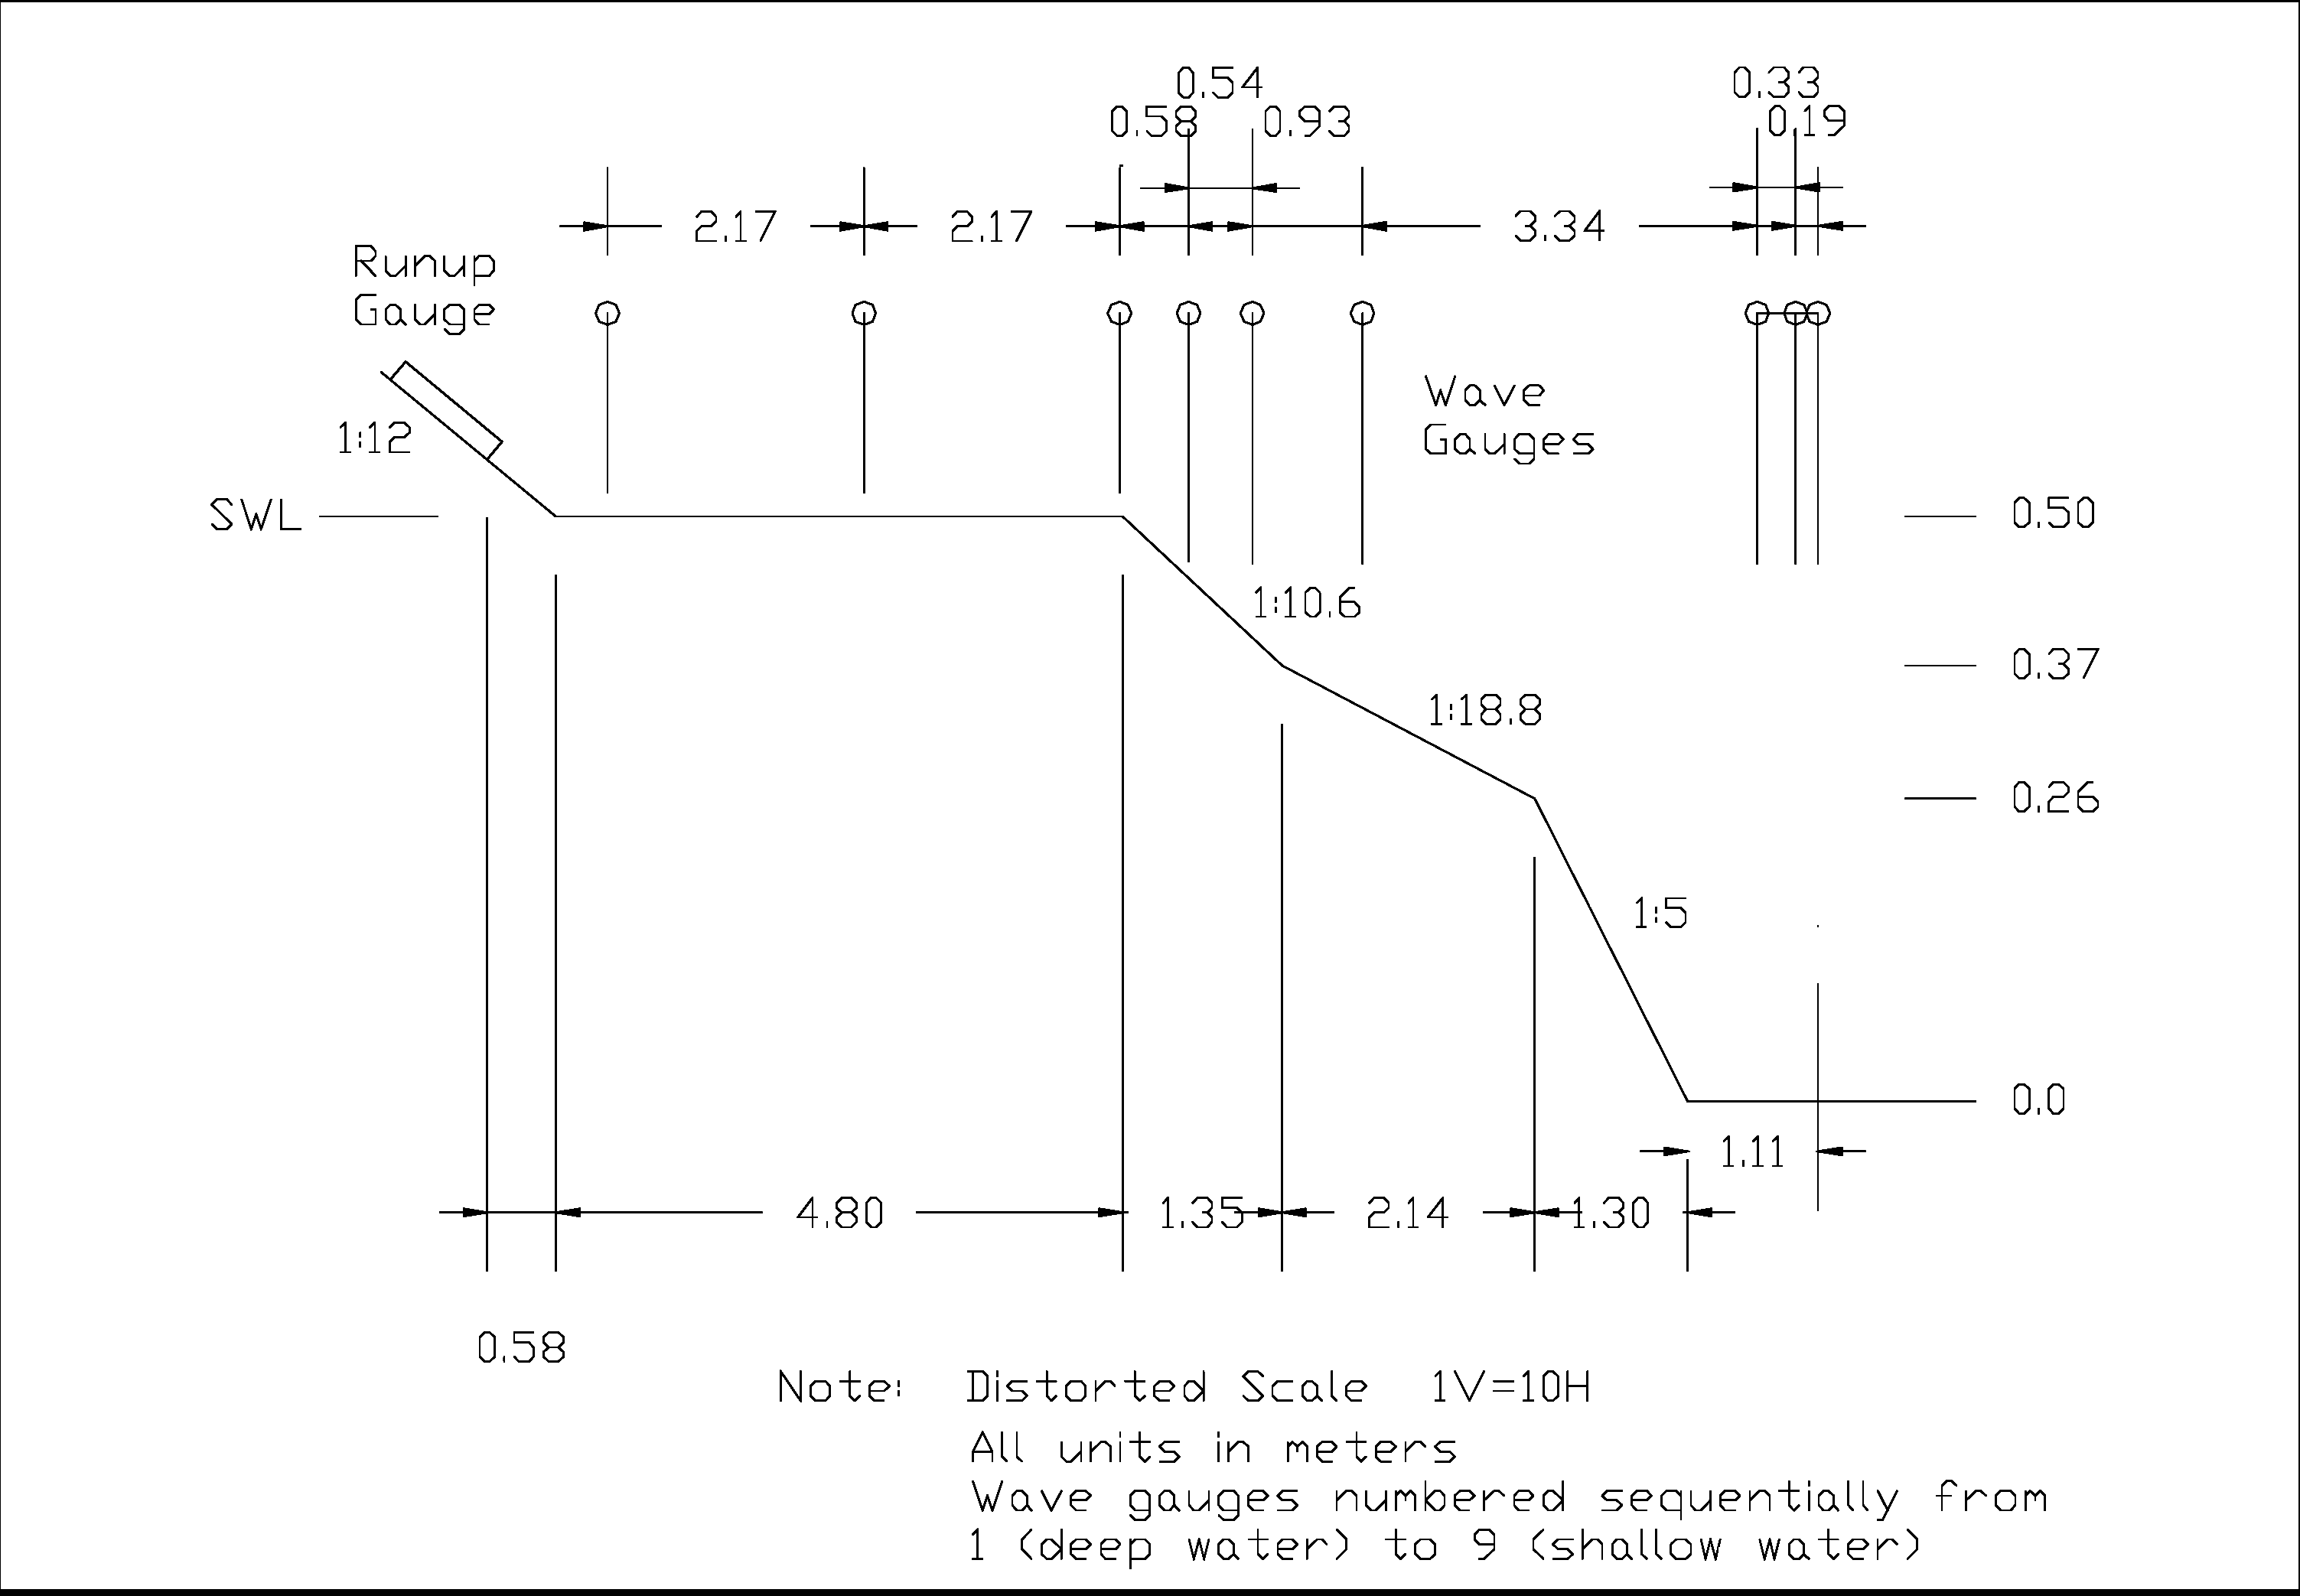
\includegraphics[scale=0.15]{./images/instrumen_eksperimen.png}
  \end{center}
  \caption{Instrumen eksperimen yang digunakan oleh Demirbilek et al \cite{DemirbilekReport}.}
  \label{fig:intrumen_demirbilek}
\end{figure}

Gambar \ref{fig:intrumen_demirbilek} merupakan konfigurasi yang digunakan Demirbilek et al \cite{DemirbilekReport} untuk mengamati gelombang. Pada konfigurasi tersebut ada 9 sensor gelombang, 2 sensor kecepatan angin, dan 1 sensor \emph{runup} gelombang. Wilayah penyebaran sensor gelombang dikelompokan menjadi 2. Wilayah pertama berada di atas karang dan wilayah kedua berada di laut. Wilayah karang merupakan gabungan dari wilayah karang yang datar \emph{Reef Flat} dan wilayah karang yang miring. Wilayah karang datar memiliki panjang mulai dari \emph{SWL} hingga 4.8 meter ke arah laut. Wilayah karang yang miring \emph{Reef Slope} di mulai dari bibir karang datar hingga 4.79 meter ke arah laut. Laut didefinisikan dengan wilayah dengan dasar terdalam. Untuk sensor 1, 2, dan 3 tersebar di wilayah laut, sensor 4, 5, dan 6 tersebar di wilayah \emph{reef slope}, dan untuk sensor 7, 8, dan 9 tersebar di wilayah \emph{reef flat}. Dengan demikian, sensor yang digunakan untuk prediktor pada jurnal ini adalah sensor 1, 2, dan 3.

\subsection{Optimasi Hyperparameter}
\begin{table}[h]
  \begin{center}
    \begin{tabular}{lrrrr}
      \toprule
      Parameter &        Interval Nilai \\
      \midrule
      Hidden Layer            & {[}1, 5{]}     \\
      Neuron per Layer        & \{0.5LookBack, 0.5LookBack, 1LookBack\}    \\
      Prediktor               & \{1, 3\}       \\
      Epoch                   & {[}100, 500, 800{]} \\
      Model Prediktor         & \{Time Series, Non Time Series\} \\
      LookBack (Time Series)  & {[}7.5 Detik, 15 Detik, 30 Detik{]}\\
      \bottomrule
    \end{tabular}
  \end{center}
  \caption{Tabel batasan pencarian hyperparameter}\label{tab:batasanParameter}
\end{table}

Pembangunan sistem dimulai dengan melakukan optimasi \emph{hyperparameter}. Hyperparameter yang dicari pada proses ini adalah jumlah prediktor, jumlah hidden layer, jumlah neuron, dan jumlah epoch. Karna hyperparameter pada ANN tidak memiliki batasan, maka proses pencarian parameter dibatasi. Batasan-batasan pada parameter, secara lengkap ada pada Tabel \ref{tab:batasanParameter}. Metrik yang digunakan untuk melihat performa dari parameter adalah MAPE. Metode yang digunakan pada \emph{hyperparameter tuning} pada jurnal ini adalah \emph{random search} \cite{bergstra_random_nodate}.

Tujuan dari proses optimasi hyperparameter adalah untuk mencari model yang optimal dari segi penggunaan memori, waktu komputasi, dan akurasi. Semakin banyak hyperparameter yang digunakan, semakin besar pula memori dan waktu komputasi.

\subsection{Model Artificial Neural Network}
Dalam penelitian ini digunakan model ANN dengan 1 output dengan fungsi aktivasi linear (model regresi). Terdapat 3 input, yang berupa vektor dengan masing-masing nilai merupakan sensor 1, sensor 2, dan sensor 3 yang terletak pada laut dalam. Model AAN ini memiliki 1 output dan merupakan model \emph{regressi linear}. Output merupakan prediksi ketinggian \emph{runup} dengan satuan $cm$. Model tersebut direpresentasikan pada Gambar \ref{fig:model_ann_ta_ini}.

% \FloatBarrier
\def\layersep{4cm}
\begin{figure}[htp]
  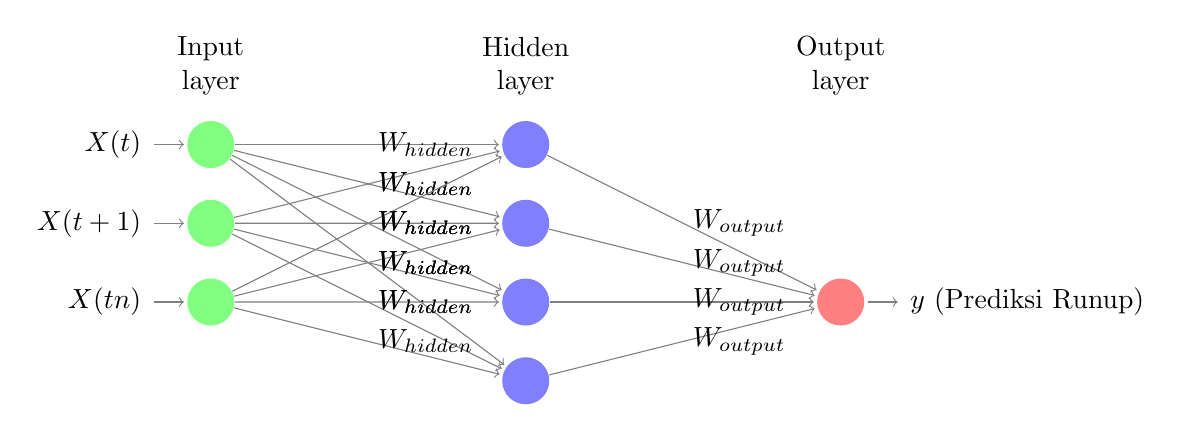
\begin{tikzpicture}[shorten >=1pt,->,draw=black!50, node distance=\layersep]
      \tikzstyle{every pin edge}=[<-,shorten <=1pt]
      \tikzstyle{neuron}=[circle, fill=black!25,minimum size=17pt,inner sep=0pt]
      \tikzstyle{input neuron}=[neuron, fill=green!50];
      \tikzstyle{output neuron}=[neuron, fill=red!50];
      \tikzstyle{hidden neuron}=[neuron, fill=blue!50];
      \tikzstyle{annot} = [text width=4em, text centered]

      % Draw the input layer nodes
      \node[input neuron, pin=left:$X(t)$] (I-SENSOR1) at (0,-1) {};
      \node[input neuron, pin=left:$X(t+1)$] (I-SENSOR2) at (0,-2) {};
      \node[input neuron, pin=left:$X(tn)$] (I-SENSOR3) at (0,-3) {};

      % Draw the hidden layer nodes
      \path[yshift=0.0cm]{}
          node[hidden neuron] (H-1) at (\layersep,-1 cm) {};
      \path[yshift=0.0cm]{}
          node[hidden neuron] (H-2) at (\layersep,-2 cm) {};
      \path[yshift=0.0cm]{}
          node[hidden neuron] (H-3) at (\layersep,-3 cm) {};
      \path[yshift=0.0cm]{}
          node[hidden neuron] (H-4) at (\layersep,-4 cm) {};

      % Draw the output layer node
      \node[output neuron,pin={[pin edge={->}]right:$y$ (Prediksi Runup)}, right of=H-3] (O) {};

      % Connect every node in the input layer with every node in the
      % hidden layer.
      \foreach \source in {SENSOR1, SENSOR2, SENSOR3}
          \foreach \dest in {1,...,4}
              \path (I-\source) edge node[midway, right] {$W_{hidden}$} (H-\dest);

      % Connect every node in the hidden layer with the output layer
      \foreach \source in {1,...,4}
          \path (H-\source) edge node[midway, right] {$W_{output}$} (O);

      % Annotate the layers
      \node[annot,above of=H-1, node distance=1cm] (hl) {Hidden layer};
      \node[annot,left of=hl] {Input layer};
      \node[annot,right of=hl] {Output layer};
      \label{modelANNTA}
  \end{tikzpicture}
  \caption{Model ANN yang digunakan pada jurnal ini. $X$ adalah matriks dari Sensor 1 (prediktor), dan $y$ adalah hasil prediksi.}
  \label{fig:model_ann_ta_ini}
\end{figure}
\FloatBarrier


% \subsection{Flowchart Sistem TA}

% Secara keseluruhan, terdapat bentuk hirarki dalam sistem ini. Hirarki \emph{root} (Hirarki Utama), yakni sistem itu sendiri, bertugas sebagai pengatur. \emph{Root} memiliki anak yang memiliki tugas-tugas tertentu, seperti: \emph{Membaca File}, \emph{Transformasi Data}, \emph{Membagi Data}, atau yang paling penting yakni \emph{Training Data}.

\subsection{Flowchart Sistem}

Sistem utama merupakan pengatur dari komponen-komponen yang ada pada sistem jurnal ini. Komponen-komponen tersebut termasuk: Pembacaan Data, Transformasi Data, Pembagian Data,Inisialisasi Epoch Dan Learning Rate, Melakukan Training, dan Melakukan Testing. Alur kerja lebih lanjut dapat dilihat pada Gambar \ref{fig:flowchart_sistem}.

Sistem utama dimulai dengan membaca data. Pembacaan data dibagi menjadi 2. Pembacaan data training dan pembacaan data testing. Data training mencakup 80 persen dari seluruh data observasi, sedangkan data training mencakup 20 persen. Hal ini sejalan dengan Fan et al \cite{fan2008liblinear}, dimana beliau menggunakan rasio 80/20 untuk training dan testing. Setelah melakukan pembacaan data, sistem akan melakukan transformasi data. Mengubah data csv, menjadi matriks dengan panjang kolom yang mewakili nilai dari prediktor. Komponen selanjutnya adalah inisialisasi \emph{epoch} dan \emph{learning rate}. \emph{Epoch} adalah representasi dari keseluruhan data yang digunakan pada training. Sedangkan \emph{learning rate} adalah besaran dari suatu langkah pembelajaran. Nilai dari \emph{learning rate} dan \emph{epoch} selanjutnya akan dimasukan ke dalam fungsi training.

\begin{figure}[ht]
  \caption{Flowchart Sistem Utama}
  \begin{center}
    \tikzstyle{decision} = [diamond, draw, 
        text width=4.5em, text badly centered, node distance=3cm, inner sep=0pt]
    \tikzstyle{block} = [rectangle, draw, 
        text width=12em, text centered, minimum height=2em]
    \tikzstyle{circle} = [draw, ellipse, minimum height=2em, distance=4em]
    \tikzstyle{blockTraining} = [rectangle, draw, fill=red!20, 
        text width=12em, text centered, minimum height=2em]
    \tikzstyle{line} = [draw, -latex']
        
    \begin{tikzpicture}[node distance = 1.5cm, auto]
        \footnotesize
        % Place nodes
        \node [circle] (init) {Mulai};
        \node [block, below of=init] (bacaData) {Membaca data report dari csv file};
        \node [block, below of=bacaData] (transformasiData) {Transformasi data menjadi matrix};
        \node [block, below of=transformasiData] (setupEpochLr) {Menentukan jumlah epoch dan learning rate};
        \node [blockTraining, below of=setupEpochLr] (training) {Melakukan Training};
        \node [blockTraining, below of=training] (testing) {Melakukan Testing};
        \node [circle, below of=testing] (stop) {Stop};
      
        % Draw edges
        \path [line] (init) -- (bacaData);
        \path [line] (bacaData) -- (transformasiData);
        \path [line] (transformasiData) -- (setupEpochLr);
        \path [line] (setupEpochLr) -- (training);
        \path [line] (training) -- (testing);
        \path [line] (testing) -- (stop);
        \label{fig:sistem}
    \end{tikzpicture}
  \end{center}
  \label{fig:flowchart_sistem}
\end{figure}
\FloatBarrier

\subsubsection{Flowchart Komponen Training Dan Testing}
\label{FlowChartTraining}

Pada bagian training dan testing (Gambar \ref{fig:sistem}), algoritma yang digunakan adalah algoritma ANN. Untuk testing, hanya dilakukan algoritma \emph{Feed Forward}. Alur kerja ANN direpresentasikan pada Gambar \ref{fig:alur_ann}.

\begin{figure}[ht]
  \caption{Flowchart Komponen Training Dan Testing}
  \begin{center}
    \footnotesize
    \tikzstyle{block} = [rectangle, draw, fill=blue!20, 
        text width=10em, text centered, minimum height=6em]
    \tikzstyle{blockTraining} = [rectangle, draw, fill=red!20, 
        text width=14em, text centered, minimum height=2em]
    \tikzstyle{stopTrainng} = [rectangle, draw, fill=red!20, 
        text width=3em, text centered,  distance=10cm]
    \tikzstyle{line} = [draw, -latex']
    \tikzstyle{circle} = [draw, ellipse, minimum height=2em, distance=4em]
    \tikzstyle{decision} = [diamond, draw, fill=blue!20, 
        text width=4em, text badly centered, node distance=2.5cm, inner sep=0pt]
        
    \begin{tikzpicture}[node distance = 1.5cm, auto]
        % Place nodes
        \node [circle] (init) {Mulai};
        \node [blockTraining, below of=init] (randomWeight) {Inisialisasi $weight$ dengan random data};
        \node [blockTraining, below of=randomWeight] (IW){Mengalikan Input Layer Dengan $Weight$ hidden layer};
        \node [blockTraining, below of=IW] (aktivasi){Jalankan fungsi aktivasi hidden layer};
        \node [blockTraining, below of=aktivasi] (HW){Mengalikan Input Layer Dengan $Weight$ untuk $output$};
        \node [blockTraining, below of=HW] (aktivasiOutput){Menjalankan fungsi aktivasi untuk output neuron};
        \node [blockTraining, below of=aktivasiOutput] (cost){Kalkulasi Error};
        \node [circle, below of=cost] (stop){Stop};
  
        % Draw edges
        \path [line] (init) -- (randomWeight);
        \path [line] (randomWeight) -- (IW);
        \path [line] (IW) -- (aktivasi);
        \path [line] (aktivasi) -- (HW);
        \path [line] (HW) -- (aktivasiOutput);
        \path [line] (aktivasiOutput) -- (cost);
        \path [line] (cost) -- (stop);
    \end{tikzpicture}
  \end{center}
  \label{fig:alur_ann}
\end{figure}
\FloatBarrier

Pada Gambar \ref{fig:alur_ann}, algoritma ANN dimulai dengan inisialisasi weight dengan random data(data acak). Selanjutnya, nilai pada \emph{input layer} akan dikalikan dengan $weight$ \emph{hidden layer}, sehingga dihasilkan $a^1$. Untuk menjadi nilai pada \emph{neuron hidden layer} $z^1$, $a$ akan diaktifasi dengan fungsi aktivasi $RELU$ sehingga nilai $z^1$ merupakan hasil dari $relu(a)$. Untuk mengahasilkan nilai prediksi, $z^1$ dikalikan dengan $weight$ pada \emph{output} $W^2$, sehingga mengasilkan $a^2$. Nilai $a^2$ merupakan nilai hasil prediksi, karna fungsi aktivasi dari \emph{output} adalah linear ($f(a) = a$). Lihat Gambar \ref{fig:model_ann_ta_ini} untuk representasi dari Model ANN yang digunakan pada jurnal ini.

\FloatBarrier


\section{Evaluasi}
\subsection{Hasil Pengujian}
Sebagian dari hasil prediksi pada data testing dengan model yang optimal (berdasarkan percobaan) bisa dilihat pada tabel berikut:

\begin{table}[h]
  \caption{Tabel Hasil Prediksi}
  \begin{center}
    \begin{tabular}{lrr}
\toprule
Nomor Data & Observasi  &  Prediksi \\
\midrule
0 &  2.204360 &  1.627366 \\
1 &  2.093506 &  2.058117 \\
2 &  1.138201 &  1.354414 \\
3 &  1.103641 &  1.186836 \\
4 &  0.582951 &  0.731976 \\
5 &  0.413409 &  0.900809 \\
6 &  0.500462 &  0.060684 \\
7 &  0.316248 &  0.878779 \\
8 &  0.482204 &  0.093842 \\
9 &  1.183195 &  0.923174 \\
\bottomrule
\end{tabular}

  \end{center}
  \label{tab:hasilPengujianLengkap10}
\end{table}

\FloatBarrier
\noindent Hasil prediksi pada data testing hingga data ke 50 terlampir pada Table \ref{tab:hasilPengujianLengkap}. Untuk melihat hasil benchmark setiap konfigurasi model, bisa dilihat pada Tabel \ref{tab:hypertunningTest}, Tabel \ref{tab:hypertunningTrain}, dan Tabel \ref{tab:hypertunningVal}.

\subsection{Analisis Hasil Pengujian}

Sistem diuji terhadap data percobaan nomor 18 (dengan nama file "test-18.dat"). Pengujian dilakukan pada sensor 1 (Wave 1) sebagai prediktor. Data tersebut dirata-ratakan dengan metode moving average pada setiap 8 data. Untuk target prediksi digunakan kolom "Wave9" (Sensor 9).

Proses pertama yang dilakukan adalah proses optimasi \emph{hyperparameter}. Metode yang digunakan adalah grid search. Batasan-batasan untuk pencarian \emph{hyperparameter} optimal yang dilakukan pada jurnal ini ada pada Tabel \ref{tab:batasanParameter}.

Metrik yang digunakan pada optimasi \emph{hyperparameter} adalah $MSE$ dengan input menggunakan data testing, yang memiliki jumlah 15 persen dari total data. Dari proses tersebut diraih model optimal, denhan konfigurasi sebagai berikut:
\FloatBarrier
\begin{table}[h]
  \caption{Tabel Konfigurasi}
  \label{tab:modelOptimal}
  \begin{center}
    \begin{tabular}{lrrrr}
      \toprule
      Parameter &        Interval Nilai \\
      \midrule
      Hidden Layer            & 5    \\
      Neuron per Layer        & 120    \\
      Prediktor               & 120    \\
      Epoch                   & 800  \\
      Model Prediktor         & Time Series \\
      LookBack (Time Series)  & 15 Detik \\
      % Stationary?
      \bottomrule
    \end{tabular}
  \end{center}
\end{table}
\FloatBarrier
\noindent Model pada Tabel \ref{tab:modelOptimal} memiliki nilai $MSE$ pada data testing sebesar $0.01130502743837540$, sedangkan pada data training memiliki nilai $MSE$ sebesar $0.024987277789757800$ pada epoch ke 800.
\FloatBarrier
\begin{figure}[h]
  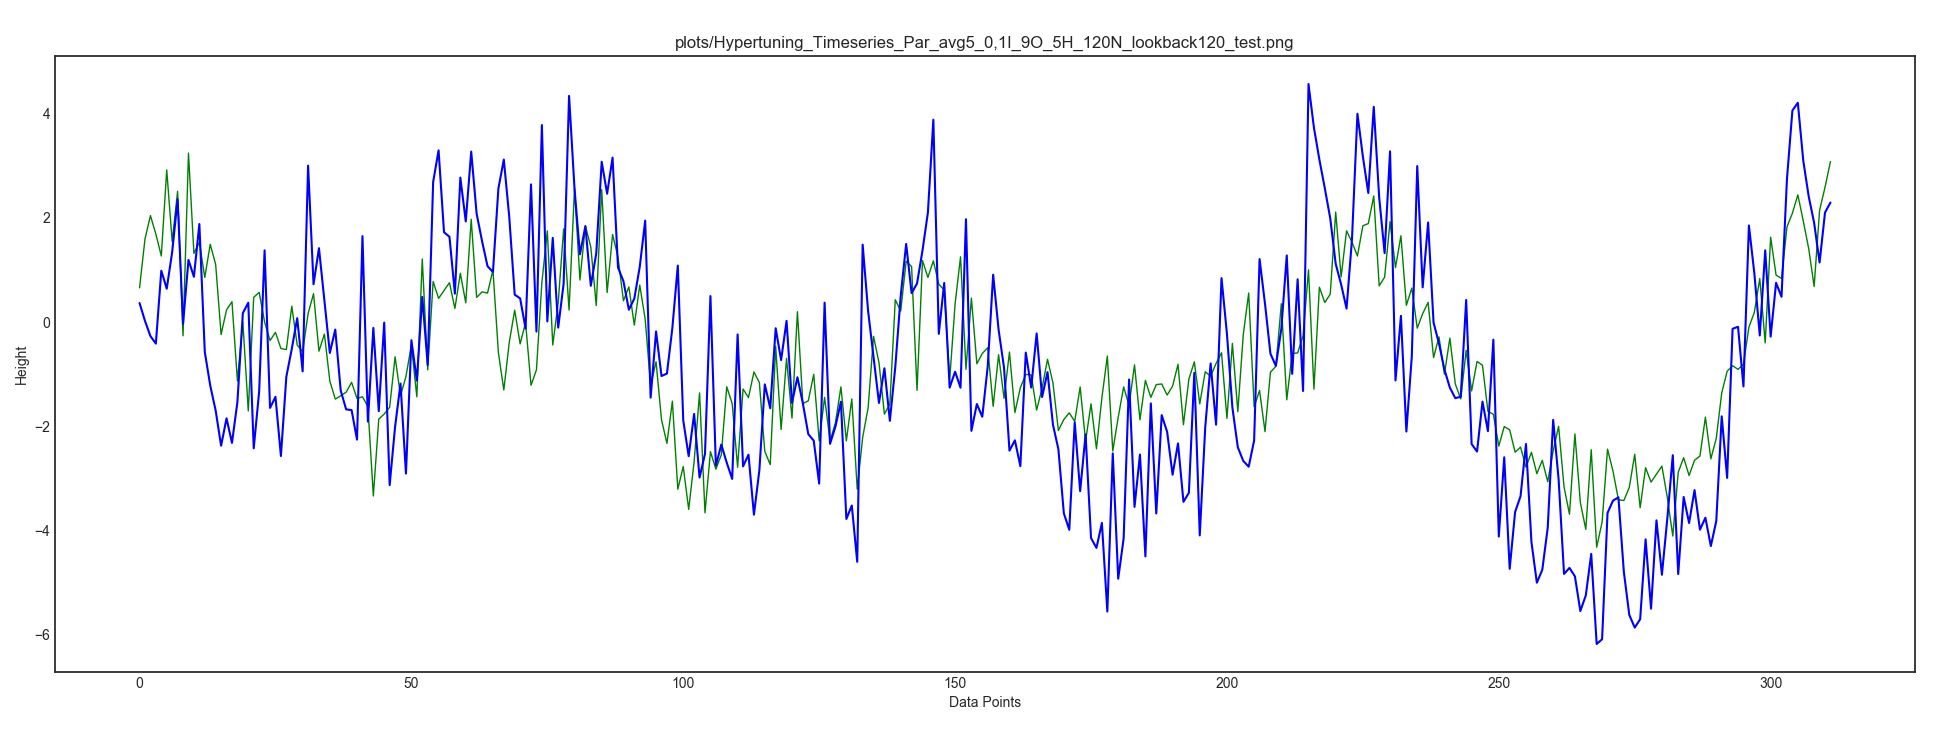
\includegraphics[scale=0.34]{./images/Hypertuning_Timeseries_Par_avg5_0,1I_9O_5H_120N_lookback120_test.png}
  \caption{Plot perbandingan observasi dan prediksi pada data testing. Hijau adalah observasi dan biru adalah prediksi. Prediktor yang digunakan adalah sensor 1 (Wave1), dan targetnya adalah sensor 9 (Wave 9)}
  \label{fig:perbandinganTestTerbaik}
\end{figure}

\begin{figure}[h]
  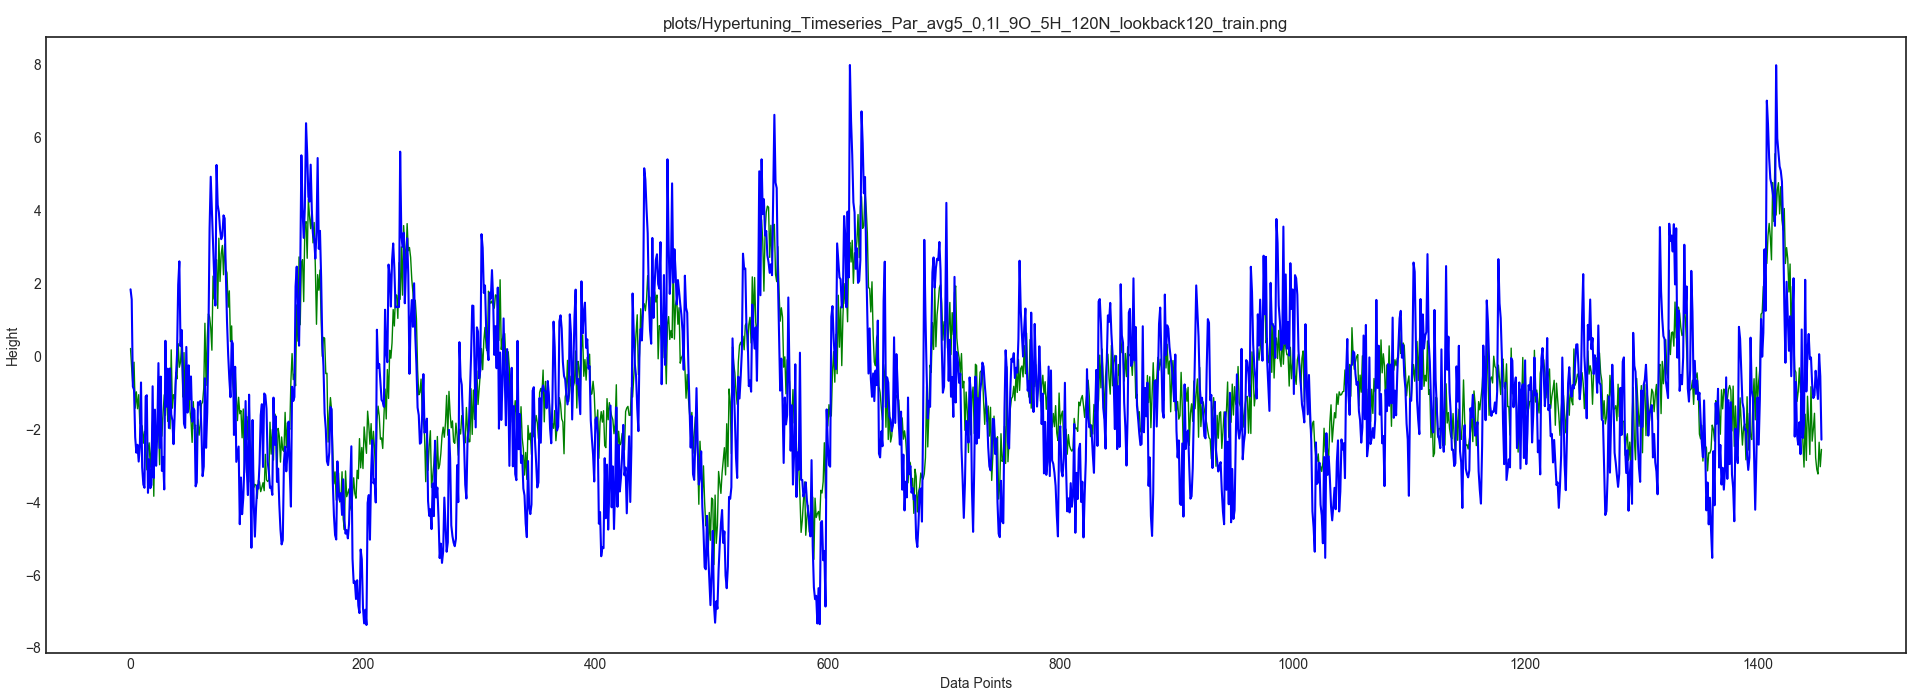
\includegraphics[scale=0.34]{./images/Hypertuning_Timeseries_Par_avg5_0,1I_9O_5H_120N_lookback120_train.png}
  \caption{Plot perbandingan observasi dan prediksi pada data training. Hijau adalah observasi dan biru adalah prediksi. Prediktor yang digunakan adalah sensor 1 (Wave1), dan targetnya adalah sensor 9 (Wave 9)}
  \label{fig:perbandinganTrainTerbaik}
\end{figure}
\FloatBarrier
Perbandingan nilai observasi dan nilai prediksi untuk data training dapat dilihat di Gambar \ref{fig:perbandinganTestTerbaik}. Bila dibandingkan dengan Gambar \ref{fig:perbandinganTrainTerbaik}, dapat dilihat terjadi overfitting. Rasio perbedaan $MSE$ pada training dan testing adalah $1:2.2$.

Merujuk pada Tabel \ref{tab:hypertunningTest}, dapat dilihat bahwa $80\%$ dari $10$ model dengan nilai $MSE$ terkecil adalah model dengan jumlah \emph{hidden layer} 5. Sedangkan untuk \emph{hyperparameter} \emph{lookback}, dari $10$ model dengan nilai $MSE$ terkecil, terdapat 4 model dengan nilai \emph{lookback} 120.

\section{Kesimpulan}
Proses optimasi \emph{hyperparameter} pada prediksi \emph{runup} gelombang sangat penting untuk membangun model pada jurnal ini. Pada proses itu menghasilkan konfigurasi model yang optimal dari parameter-parameter yang sudah ditentukan sebelumnya. Model yang optimal pada percobaan di jurnal ini adalah model dengan 5 \emph{hidden layer}, 120 \emph{neuron}, dan 120 \emph{lookback}. Model tersebut memiliki nilai $MSE$ sebesar $0.011305$. Karena terdapat rasio $1:2.2$ pada data testing, model tersebut dapat dikatakan \emph{overfitting}. Meskipun nilai $MSE$ yang dihasilkan merupakan nilai $MSE$ yang terbaik pada data testing dibandingkan konfigurasi parameter lainnya.

% hasil dari penelitian ini masih 
% Hasil dari pemodel machine learning dalam penelitian ini masih belum mengalahkan pemodelan numerik dari sisi akurasi. Namun demikian, masih tersedia ruang untuk pengembangan yang sangat besar. Mengingat waktu komputasi proses prediksi machine learning lebih cepat dari pada metode lainnya.  

% \subsection{Saran}
% Ada jenis lain dari \emph{neural network} yang mampu mengingat output dari $T - 1$ dan memasukannya sebagai parameter untuk komputasi output saat ini, disebut dengan $Recurent Neural Network (RNN)$ \cite{werbos1990backpropagation}.
% Dan pada tahun 1997, Sepp Hochreiter dan Jürgen Schmidhuber mempblikasikan paper tentang \emph{Long Short-term Memory}\cite{lstm1997}, yang bisa dijadikan alternative solusi dari masalah \emph{Vanishing Gradient dan Decaying Gradient} yang terkadang timbul dalam pengaplikasian model $RNN$.

\bibliographystyle{abbrv}
\bibliography{references}
\pagebreak
\section*{Lampiran}

\begin{figure}[h]
  \includepdf{plots/sensor-1-9-test18.pdf}
  \label{fig:plots_semua_sensor_test18}
  \caption{Plot sensor 1 hingga sensor 10.}
\end{figure}
\pagebreak

\begin{table}[h]
  \caption{Tabel Hasil Dari Optimasi \emph{HyperParameter} Untuk Data Testing}
  \begin{center}
    \begin{tabular}{lrrrrrr}
\toprule
{} &  Hidden Layer &  Neurons &  Lookback &  Test MSE &  Test Mape &     Test R\textasciicircum 2 \\
\midrule
0  &             5 &      120 &       120 &  0.011305 &  26.414053 &    -0.264644 \\
1  &             5 &       48 &        60 &  0.012787 &  27.174426 &  -143.859941 \\
2  &             5 &       60 &        60 &  0.013404 &  26.781531 &   -22.040994 \\
3  &             5 &       96 &       120 &  0.013433 &  25.683588 &    -0.435304 \\
4  &             3 &       96 &       120 &  0.013798 &  29.610516 &    -0.556499 \\
5  &             5 &      192 &       240 &  0.014218 &  28.919896 &    -0.182490 \\
6  &             5 &       60 &       120 &  0.015099 &  30.136892 &    -0.731013 \\
7  &             5 &       30 &        60 &  0.015808 &  27.766505 &   -49.909962 \\
8  &             3 &      240 &       240 &  0.016168 &  31.874225 &    -0.501018 \\
9  &             5 &      240 &       240 &  0.016528 &  33.960820 &    -0.419433 \\
10 &             3 &       60 &        60 &  0.016580 &  32.164772 &  -451.287667 \\
11 &             3 &      120 &       120 &  0.016904 &  32.004432 &    -0.936859 \\
12 &             1 &       48 &        60 &  0.017205 &  33.184803 &  -842.164714 \\
13 &             1 &       60 &        60 &  0.018040 &  34.036791 &  -773.051533 \\
14 &             1 &       96 &       120 &  0.018128 &  34.060344 &    -1.047246 \\
15 &             3 &       48 &        60 &  0.018598 &  33.886219 &  -831.895232 \\
16 &             3 &       60 &       120 &  0.018676 &  34.424763 &    -1.151863 \\
17 &             1 &      120 &       120 &  0.018833 &  34.276165 &    -1.138369 \\
18 &             3 &      120 &       240 &  0.018852 &  33.463418 &    -0.636688 \\
19 &             3 &       30 &        60 &  0.019018 &  35.014525 &  -825.339841 \\
20 &             3 &      192 &       240 &  0.019159 &  33.471239 &    -0.704520 \\
21 &             5 &      120 &       240 &  0.019243 &  36.270492 &    -0.644902 \\
22 &             1 &       30 &        60 &  0.019823 &  35.997234 & -1020.453354 \\
23 &             1 &      120 &       240 &  0.020242 &  35.658058 &    -0.974649 \\
24 &             1 &      240 &       240 &  0.020375 &  36.627155 &    -0.985365 \\
25 &             1 &      192 &       240 &  0.021186 &  36.747288 &    -1.009583 \\
26 &             1 &       60 &       120 &  0.021303 &  36.555191 &    -1.402687 \\
\bottomrule
\end{tabular}

  \end{center}
  \label{tab:hypertunningTest}
\end{table}
\pagebreak

\begin{table}[h]
  \caption{Tabel Hasil Prediksi}
  \begin{center}
    \begin{tabular}{lrr}
\toprule
Data Point &  Observasi & Prediksi \\
\midrule
0  &  2.204360 &  1.627366 \\
1  &  2.093506 &  2.058117 \\
2  &  1.138201 &  1.354414 \\
3  &  1.103641 &  1.186836 \\
4  &  0.582951 &  0.731976 \\
5  &  0.413409 &  0.900809 \\
6  &  0.500462 &  0.060684 \\
7  &  0.316248 &  0.878779 \\
8  &  0.482204 &  0.093842 \\
9  &  1.183195 &  0.923174 \\
10 &  0.252996 &  0.259298 \\
11 &  0.065848 &  0.319075 \\
12 &  0.028679 &  0.481530 \\
13 &  1.029955 &  0.277669 \\
14 &  1.043323 &  0.742714 \\
15 & -0.026749 & -0.093232 \\
16 &  0.340049 &  0.542825 \\
17 &  0.024440 & -0.230294 \\
18 &  0.060957 &  0.482178 \\
19 &  1.141462 &  0.735569 \\
20 &  0.137251 &  0.169818 \\
21 &  0.885518 &  0.065398 \\
22 &  0.269950 &  0.385597 \\
23 &  0.635444 &  0.811883 \\
24 &  1.395449 &  0.925484 \\
25 &  0.464597 &  0.406527 \\
26 &  1.247426 &  0.922542 \\
27 &  0.213871 &  0.460827 \\
28 &  0.367111 &  0.579182 \\
29 &  0.010746 &  0.966335 \\
30 &  1.640307 &  0.874319 \\
31 &  0.917145 &  0.612608 \\
32 &  1.334479 &  0.732341 \\
33 &  0.684350 &  0.834274 \\
34 &  1.337739 &  1.052186 \\
35 &  0.834656 &  1.255694 \\
36 &  0.766839 &  1.114280 \\
37 &  0.506983 &  0.954462 \\
38 &  0.841177 &  0.931447 \\
39 &  1.226885 &  1.453319 \\
40 &  1.490654 &  1.319050 \\
41 &  2.255875 &  1.181492 \\
42 &  2.511166 &  1.833375 \\
43 &  1.580641 &  1.798542 \\
44 &  1.758986 &  1.507362 \\
45 &  1.221668 &  1.015057 \\
46 &  0.730974 &  0.887336 \\
47 &  0.685328 &  1.096693 \\
48 &  1.572816 &  1.645787 \\
49 &  0.852914 &  0.914307 \\
\bottomrule
\end{tabular}

  \end{center}
  \label{tab:hasilPengujianLengkap}
\end{table}
\pagebreak
\begin{sidewaystable}
  \caption{Tabel Hasil Dari \emph{HyperParameter} Tunning Untuk Data Training}
  \begin{center}
    \scalebox{.8}{\begin{tabular}{lrrrrrrrrrrrr}
\toprule
{} &  Hidden Layer &  Neurons &  Lookback &  Train E100 MSE &  Train E100 Mape &  Train E100 R\textasciicircum 2 &  Train E500 MSE &  Train E500 Mape &  Train E500 R\textasciicircum 2 &  Train E800 MSE &  Train E800 Mape &  Train E800 R\textasciicircum 2 \\
\midrule
0  &             5 &      120 &       120 &        0.024987 &    280239.527108 &        0.025146 &        0.016317 &    256207.632661 &        0.357668 &        0.010702 &    200856.004298 &        0.572547 \\
1  &             5 &       48 &        60 &        0.024857 &    249016.834728 &        0.021211 &        0.017778 &    242268.621029 &        0.290238 &        0.013386 &    226045.459257 &        0.451499 \\
2  &             5 &       60 &        60 &        0.025305 &    294011.212876 &        0.005396 &        0.018826 &    287700.880362 &        0.244910 &        0.013422 &    261507.489104 &        0.448512 \\
3  &             5 &       96 &       120 &        0.025537 &    295846.156303 &        0.002593 &        0.017798 &    272912.219216 &        0.292762 &        0.011554 &    199410.721228 &        0.540794 \\
4  &             3 &       96 &       120 &        0.025319 &    288874.587707 &        0.011555 &        0.018098 &    264855.275925 &        0.282567 &        0.013073 &    228018.176666 &        0.484635 \\
5  &             5 &      192 &       240 &        0.025854 &    285785.550983 &        0.030428 &        0.015950 &    216519.202572 &        0.391859 &        0.010548 &    161187.783747 &        0.603495 \\
6  &             5 &       60 &       120 &        0.025941 &    240665.292375 &       -0.006810 &        0.020432 &    232654.224082 &        0.191511 &        0.013017 &    176464.167031 &        0.484873 \\
7  &             5 &       30 &        60 &        0.024126 &    304655.747045 &        0.042785 &        0.018017 &    295866.444764 &        0.280452 &        0.015303 &    275814.032234 &        0.379279 \\
8  &             3 &      240 &       240 &        0.025865 &    324232.961543 &        0.023376 &        0.017607 &    281006.264564 &        0.336938 &        0.012211 &    240688.104029 &        0.536998 \\
9  &             5 &      240 &       240 &        0.025500 &    309833.417931 &        0.037378 &        0.015333 &    225568.486100 &        0.419356 &        0.009510 &    153527.980700 &        0.631424 \\
10 &             3 &       60 &        60 &        0.025121 &    268268.420056 &       -0.008522 &        0.021447 &    268938.490083 &        0.160475 &        0.017750 &    262793.014663 &        0.277893 \\
11 &             3 &      120 &       120 &        0.026766 &    300349.932862 &       -0.048153 &        0.020989 &    275588.518647 &        0.170371 &        0.016091 &    232788.210306 &        0.366387 \\
12 &             1 &       48 &        60 &        0.024962 &    268749.745084 &        0.018043 &        0.021124 &    273507.998781 &        0.165314 &        0.018916 &    274400.476088 &        0.245280 \\
13 &             1 &       60 &        60 &        0.025403 &    269035.103046 &       -0.006477 &        0.021622 &    276602.140189 &        0.142863 &        0.019365 &    276751.674388 &        0.229592 \\
14 &             1 &       96 &       120 &        0.025667 &    284167.313229 &        0.006787 &        0.021474 &    273618.079339 &        0.154057 &        0.018982 &    258967.098817 &        0.254853 \\
15 &             3 &       48 &        60 &        0.025051 &    279736.602346 &       -0.000561 &        0.022409 &    279534.747945 &        0.117154 &        0.019670 &    276377.085081 &        0.214018 \\
16 &             3 &       60 &       120 &        0.025902 &    303814.329584 &       -0.021078 &        0.022048 &    287044.487247 &        0.144393 &        0.018275 &    268736.329922 &        0.285089 \\
17 &             1 &      120 &       120 &        0.025250 &    272145.554569 &        0.026243 &        0.020968 &    267600.687003 &        0.173897 &        0.018565 &    249460.240715 &        0.269657 \\
18 &             3 &      120 &       240 &        0.025750 &    299551.389564 &        0.034315 &        0.018194 &    266379.875698 &        0.322110 &        0.012600 &    211614.776995 &        0.523712 \\
19 &             3 &       30 &        60 &        0.025634 &    269018.098708 &       -0.026156 &        0.023064 &    277227.123537 &        0.089592 &        0.020583 &    277668.186370 &        0.175067 \\
20 &             3 &      192 &       240 &        0.026306 &    269103.678175 &        0.013316 &        0.019078 &    240496.562848 &        0.290748 &        0.013609 &    187956.220897 &        0.488481 \\
21 &             5 &      120 &       240 &        0.026730 &    278333.471970 &       -0.002670 &        0.017991 &    229528.398579 &        0.320574 &        0.011244 &    149991.457696 &        0.569197 \\
22 &             1 &       30 &        60 &        0.025825 &    284193.575632 &       -0.018582 &        0.023180 &    281111.385021 &        0.085725 &        0.021401 &    283876.147566 &        0.149779 \\
23 &             1 &      120 &       240 &        0.027504 &    324770.492283 &       -0.026773 &        0.021996 &    293764.156883 &        0.186267 &        0.018990 &    277863.111062 &        0.283659 \\
24 &             1 &      240 &       240 &        0.026450 &    298939.539037 &        0.006474 &        0.020706 &    284665.626925 &        0.229160 &        0.017614 &    265786.215927 &        0.333985 \\
25 &             1 &      192 &       240 &        0.026445 &    288148.087104 &        0.011977 &        0.021324 &    274522.370043 &        0.210871 &        0.018297 &    259969.908423 &        0.309053 \\
26 &             1 &       60 &       120 &        0.026652 &    272469.263962 &       -0.029809 &        0.023513 &    266514.870440 &        0.088461 &        0.021530 &    255857.454129 &        0.151129 \\
\bottomrule
\end{tabular}
}
  \end{center}
  \label{tab:hypertunningTrain}
\end{sidewaystable}
\pagebreak
\begin{sidewaystable}
  \caption{Tabel Hasil Dari HyperParameter Tunning Untuk Data Validasi}
  \begin{center}
    \scalebox{.8}{\begin{tabular}{lrrrrrrrrrrrr}
\toprule
{} &  Hidden Layer &  Neurons &  Lookback &  Val E100 MSE &  Val E100 Mape &  Val E100 R\textasciicircum 2 &  Val E500 MSE &  Val E500 Mape &  Val E500 R\textasciicircum 2 &  Val E800 MSE &  Val E800 Mape &  Val E800 R\textasciicircum 2 \\
\midrule
0  &             5 &      120 &       120 &      0.044993 &      96.021665 &     -1.179030 &      0.027930 &      74.308036 &     -0.430468 &      0.019560 &      60.183270 &     -0.032957 \\
1  &             5 &       48 &        60 &      0.042760 &      93.178239 &  -1752.373489 &      0.026447 &      66.240550 &  -1261.139921 &      0.018534 &      42.859303 &   -747.342139 \\
2  &             5 &       60 &        60 &      0.043575 &      94.377521 &  -1678.115619 &      0.028496 &      72.011074 &  -1202.088144 &      0.018805 &      44.877317 &   -539.130189 \\
3  &             5 &       96 &       120 &      0.046219 &      94.883925 &     -1.223605 &      0.033132 &      74.913612 &     -0.611088 &      0.025457 &      55.896219 &     -0.189004 \\
4  &             3 &       96 &       120 &      0.045517 &      96.951947 &     -1.187200 &      0.031005 &      79.380137 &     -0.531072 &      0.021991 &      69.757003 &     -0.143614 \\
5  &             5 &      192 &       240 &      0.041200 &      79.825803 &     -1.185281 &      0.032176 &      65.187451 &     -0.740613 &      0.028327 &      62.175225 &     -0.639378 \\
6  &             5 &       60 &       120 &      0.047072 &      97.562523 &     -1.281361 &      0.037150 &      83.821622 &     -0.865156 &      0.024870 &      63.158551 &     -0.311375 \\
7  &             5 &       30 &        60 &      0.043612 &      86.327002 &  -1912.192553 &      0.031953 &      55.785185 &  -1096.096087 &      0.029813 &      45.150231 &   -529.458809 \\
8  &             3 &      240 &       240 &      0.043889 &      86.751455 &     -1.275956 &      0.035230 &      71.642604 &     -0.844360 &      0.029400 &      63.280302 &     -0.602915 \\
9  &             5 &      240 &       240 &      0.043688 &      84.619347 &     -1.262451 &      0.032495 &      68.378794 &     -0.717169 &      0.027862 &      68.584949 &     -0.585432 \\
10 &             3 &       60 &        60 &      0.043341 &      91.212592 &  -1536.188002 &      0.035014 &      79.209373 &  -1308.322015 &      0.027155 &      63.629266 &  -1015.238854 \\
11 &             3 &      120 &       120 &      0.047951 &      99.320371 &     -1.330781 &      0.036998 &      81.159244 &     -0.821370 &      0.027555 &      67.078853 &     -0.385190 \\
12 &             1 &       48 &        60 &      0.043984 &      94.376710 &  -1613.101289 &      0.035208 &      82.577577 &  -1328.965648 &      0.030118 &      74.374408 &  -1151.803761 \\
13 &             1 &       60 &        60 &      0.043846 &      93.001325 &  -1643.837491 &      0.035248 &      81.456332 &  -1446.063805 &      0.030250 &      72.978736 &  -1344.128531 \\
14 &             1 &       96 &       120 &      0.045333 &      96.988215 &     -1.161457 &      0.037497 &      86.218531 &     -0.802206 &      0.032233 &      81.817882 &     -0.563602 \\
15 &             3 &       48 &        60 &      0.044525 &      93.106114 &  -1601.699843 &      0.038695 &      83.510727 &  -1439.131395 &      0.032535 &      72.025332 &  -1214.552233 \\
16 &             3 &       60 &       120 &      0.048463 &      95.796487 &     -1.342336 &      0.040275 &      85.306509 &     -0.993697 &      0.032885 &      72.894188 &     -0.679436 \\
17 &             1 &      120 &       120 &      0.045788 &      94.219876 &     -1.197142 &      0.037645 &      79.123034 &     -0.849177 &      0.032278 &      73.985648 &     -0.613675 \\
18 &             3 &      120 &       240 &      0.044154 &      85.343212 &     -1.281351 &      0.035592 &      78.581370 &     -0.840172 &      0.030926 &      70.153028 &     -0.640556 \\
19 &             3 &       30 &        60 &      0.045253 &      92.101757 &  -1679.920438 &      0.039391 &      85.246216 &  -1426.725452 &      0.033869 &      75.715332 &  -1157.233881 \\
20 &             3 &      192 &       240 &      0.041597 &      83.467816 &     -1.242346 &      0.032965 &      77.834872 &     -0.790729 &      0.028652 &      71.363949 &     -0.607343 \\
21 &             5 &      120 &       240 &      0.045226 &      88.841955 &     -1.358351 &      0.036903 &      80.747338 &     -0.944565 &      0.031913 &      78.829563 &     -0.805048 \\
22 &             1 &       30 &        60 &      0.045994 &      95.091580 &  -2038.187597 &      0.039972 &      87.837998 &  -1743.380970 &      0.035780 &      82.113201 &  -1581.221094 \\
23 &             1 &      120 &       240 &      0.047179 &      86.500875 &     -1.519832 &      0.040912 &      82.450075 &     -1.183739 &      0.037839 &      79.505045 &     -1.038246 \\
24 &             1 &      240 &       240 &      0.044818 &      80.884090 &     -1.392152 &      0.037475 &      76.033422 &     -0.974813 &      0.034058 &      72.563216 &     -0.804426 \\
25 &             1 &      192 &       240 &      0.044759 &      84.636699 &     -1.374646 &      0.037974 &      79.665690 &     -1.018873 &      0.034429 &      76.084728 &     -0.840784 \\
26 &             1 &       60 &       120 &      0.048982 &      99.516059 &     -1.331833 &      0.042559 &      92.128637 &     -1.051477 &      0.038812 &      86.280749 &     -0.896481 \\
\bottomrule
\end{tabular}
}
  \end{center}
  \label{tab:hypertunningVal}
\end{sidewaystable}
